\cotefile{64}
\scanpage{78}
\mspage{3}
% archive foliation: 77

où $Q_0$ est un carré donné une fois pour toutes (\unsure{$k$} étant fixé\deleted{\unsure{?}}, disons, quand même), avec comme seule donnée un iso
\[
(16)\qquad \underline{\omega}_{Q_0}\deleted{\unsure{Q_0}}\simeq\mu_4^* \qquad\text{i.e. d'un \unsure{élément} de }\mu_4^*\wedge\underline{\omega}_{Q_0}
\]
i.e. un isom.
\[
(17)\qquad \mu_4^{\deleted{\unsure{*}}}\simeq\operatorname{Aut}^{+}(Q_0).
\]

Pour des raisons qui apparaîtront par la suite, le choix le plus opportun est de prendre pour $Q_0$ le carré \deleted{\unsure{ainsi} satisfaisant}\inserted{donné} (17), avec un côté fixé, dont \deleted{les extrémités}\inserted{\unsure{l'ens|l'une} des \unsure{2} extrémités} $s,s'$ \deleted{\unsure{est}} dans une corr. biunivoque avec l'ens. $\mu_4^*=\{i,i'\}$ des racines carrées de $-1$, par la condition que
\[
\deleted{\unsure{s'=i_s s}}
\]
\figure{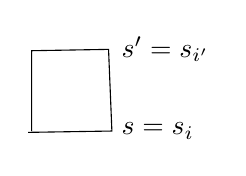
\begin{tikzpicture}[scale=.85]
\draw (0,0)--(0,1.2)--(1.15,1.22)--(1.2,0)--(-.05,-.02);
\node[anchor=west] at (1.2,1.22) {$s'=s_{i'}$};
\node[anchor=west] at (1.2,0) {$s=s_i$};
\end{tikzpicture}}
\[
(18)\qquad \deleted{\unsure{s_{i'}=}}s_{i'}=i\,s_i\qquad\text{d'où}\qquad s_i=i'\,s_{i'}
\]
puisque $i'=i^{-1}=-i$. Ainsi, $T_0$ peut s'interpréter comme \unsure{muni} de la structure \deleted{\unsure{par}}\inserted{suivante, \unsure{qui le caractérise} :} $T_0\otimes\underline{U}_{\unsure{t|4}}(-1)$ est muni d'une paire de bases, \deleted{\unsure{reliées entre}}\inserted{en corr. $1$-$1$} avec $\mu_4^*$, satisfaisant les mêmes relations (18); où maintenant le produit $i\,s_i$ est au sens de la structure vectorielle de $T_0\otimes\underline{U}_{\unsure{t|4}}(-1)$. \deleted{\unsure{Si}}

Ici on aura un iso. canonique
\[
(19)\qquad D_{Q_0}\simeq\mu_4^*
\]
et par suite la donnée (16) équivaut à la donnée d'un iso

\scanpage{79}
% archive foliation: 78
\[
(20)\qquad \alpha:\underline{\omega}_J\simeq\mu_4^*\qquad\text{i.e. d'un élément de }\underline{\omega}_J\wedge\mu_4^*.
\]

Ces définitions posées, on voit donc que la catégorie\inserted{-groupoïde} des courbes elliptiques\inserted{/$k$}, épinglées en Legendre \deleted{\unsure{sera}}\inserted{est} équivalente à la catégorie-groupoïde des \deleted{triplets couples}\inserted{triplets} $(J,t,\alpha)$ \deleted{de} formés
\[
(21)\quad\left\{\begin{array}{ll}
a)&\text{d'un ens }J\text{ à trois éléments (d'où }\Sigma_J,D_J,\Sigma_J^*\text{)}\\[4pt]
b)&\text{d'un }t\in\Sigma_J^*(k)\\[4pt]
c)&\text{d'un isom }\alpha:\underline{\omega}_J\simeq\mu_4^*\deleted{\unsure{k}}\quad(=\mu_4^*(k))
\end{array}\right.
\]

Un épinglage de Legendre-Jacobi d'échelon $2$ \inserted{d'une courbe elliptique $E$} sera la donnée d'un couple d'épinglages, l'un de Legendre, l'autre de Jacobi d'échelon $2$ i.e. d'une bijection $J\simeq\{0,1,\infty\}$, permettant d'identifier $\Sigma_J$ à la droite projective type $\mathbb{P}^1_{\unsure{k}}$. On a alors dans $\underline{\omega}_J\simeq\underline{\omega}_{\{0,1,\infty\}}$ un élément privilégié $\omega^+$, et la donnée c) \deleted{\unsure{du choix}} de l'épinglage de Legendre équivaut\inserted{donc} à celle d'une racine carrée \deleted{\unsure{choisie}} de $-1$, soit $i$ --- c'est la donnée ``arithmétique''. \deleted{Par ailleurs, la catég} La catégorie-groupoïde des courbes elliptiques sur $k$, munies d'un épinglage de Legendre-Jacobi, \deleted{équivaut à}\inserted{est rigide (pas d'auto. non identiques)} \deleted{celle des \unsure{objets} à isom. près \unsure{ce}} et elle

\scanpage{80}
\mspage{4}
% archive foliation: 79

est équivalente à celle des couples $(t,i)$, avec
\[
t\in U_{0,3}(k)=\mathbb{P}^1_k(k)\setminus\{0,1,\infty\},\quad\text{et }i\in\mu_4^*.
\]

\deleted{On peut définir sur $\Sigma_J$ le fibré}
\[
\deleted{\underline{O}_{\Sigma_J}(1)^{\unsure{\sharp}}\unsure{(}=\underline{O}_{\Sigma_J}(1)\wedge_{\unsure{\boldsymbol{\mu}|\mu}_4}}
\]
Je reviens à une base quelconque, mais je travaille en car. rés. $\ne2$ i.e. sur la base absolue\inserted{$S_0=$} $\operatorname{Spec}(\mathbb{Z}[\frac12])$. Sur \deleted{\unsure{$\Sigma_J$}} je définis, l'opération \deleted{\unsure{$\otimes$}} $\unsure{\sharp}$, sur les \deleted{\unsure{modules}} faisceaux en Modules \deleted{\unsure{sur}} sur un schéma de base $S$
\[
(22)\qquad M^{\unsure{\sharp}}=M\wedge_{\unsure{\boldsymbol{\mu}|\mu}_{4S}}\underbrace{Q_{0S}}_{\deleted{\unsure{\unsure{\boldsymbol{\mu}|\mu}}}}
\]
\margin{\uline{NB} $M^{\unsure{\sharp}}\simeq M\otimes_{\underline{O}_S}\underline{O}_S^{\unsure{\sharp}}$}
où ici on considère $Q_0$ comme un $\unsure{\boldsymbol{\mu}|\mu}_4$-torseur sur la base absolue $S_0$.

On aura donc
\[
(23)\qquad M^{\unsure{\sharp}}\otimes M^{\unsure{\sharp}}\simeq M^b\overset{\mathrm{def}}{=}M\wedge_{\unsure{\boldsymbol{\mu}|\mu}_{2S}=\{\pm1\}_S}\unsure{\boldsymbol{\mu}|\mu}_{4S}^*
\]
où
\[
\deleted{\unsure{\unsure{\boldsymbol{\mu}|\mu}_4^*\simeq}}
\]
\[
(24)\qquad\unsure{\boldsymbol{\mu}|\mu}_4^*=\unsure{\boldsymbol{\mu}|\mu}_4\setminus\unsure{\boldsymbol{\mu}|\mu}_2
\]
est considéré comme torseur sous $\unsure{\boldsymbol{\mu}|\mu}_2$, i.e. rev. étale quadratique de la base absolue $S_0$.

On s'intéresse donc, \deleted{\unsure{sur}} pour un revêtement

\scanpage{81}
% archive foliation: 80

étale $\underline{J}$ de degré $3$ sur $S$, permettant de définir un $\Sigma_J$
\[
(25)\qquad \Sigma_J=\mathbb{P}(V_{\underline{J}}(\underline{O}_S))
\]
\margin{\unsure{où}\quad\diagram{\begin{tikzcd}[column sep=small,row sep=small]
V_J(\underline{O}_S)\arrow[r,hook]&\underline{O}_S^{\underline{J}}\arrow[r,"\mathrm{tr}"]\arrow[d,equal]&\underline{O}_S\\
&p_*(\unsure{\underline{O}|\omega}_{\underline{J}})&
\end{tikzcd}} où $p:\underline{J}\mathbin{\unsure{-}}S$}
et un module inv. $\underline{O}_{\Sigma_J}(1)$, un module
\[
(26)\qquad T_{0\Sigma_J}=\underline{O}_{\Sigma_J}(1)^{\unsure{\sharp}}
\]
de sorte qu'on a un iso
\[
(27)\quad T_{0\Sigma}^{\otimes2}\simeq\underline{O}_{\Sigma_J}(2)\wedge_{\{\pm1\}}\unsure{\boldsymbol{\mu}|\mu}_4^*\simeq T_{\Sigma_J}\wedge_{\{\pm1\}}(\unsure{\boldsymbol{\mu}|\mu}_4^*\wedge\underline{\omega}_J)
\]
où $\underline{\omega}_J$ est le revêtement\inserted{étale} quadratique associé au revêtement\inserted{étale} cubique $\underline{J}$.

Si maintenant $E$ est une courbe elliptique sur la base $S$, on lui associe
\[
(28)\qquad \underline{J}=({}_2E)^*\qquad\text{rev. étale cubique de }S
\]
et on a un iso
\[
(29)\qquad E/(\pm\operatorname{id}_E)\simeq\Sigma_{\underline{J}}
\]
et un iso

\scanpage{82}
\mspage{5}
% archive foliation: 81
\[
(30)\qquad T_{E/S,0}^{\otimes2}\simeq T_{\Sigma_{\underline{J}},t}
\]
où $t$ est la section de $\Sigma_J^*=\Sigma_J\setminus D_J$ sur $S$, l'image de la section nulle de $E$. Ceci posé, on définit un \uline{épinglage de Legendre} de $E/S$ comme étant formé d'un iso
\[
(31)\quad\deleted{\unsure{T}}\underbrace{\Delta_{E/S}}_{T_{E/S,0}}\ \deleted{\unsure{\alpha}}\overset{\kappa}{\underset{\sim}{\longrightarrow}}\ \deleted{\unsure{T}}\underline{O}_{\deleted{\unsure{\Sigma_J}}}(1)_{t}^{\unsure{\sharp}}\simeq
\]
tel que \deleted{il existe un} l'isom\inserted{$\kappa^{\unsure{\otimes2|2}}$} déduit par passage au carré tensoriel s'identifie, via (30) et (27), à l'isom
\[
(32)\qquad T_{\Sigma_J,t}\simeq T_{\Sigma_J,t}\wedge_{\{\pm1\}}(\unsure{\boldsymbol{\mu}|\mu}_4^*\wedge\underline{\omega}_{\underline{J}})
\]
déduit d'une section
\[
(33)\quad\left\{\begin{array}{l}
\alpha\in\Gamma(S,\unsure{\boldsymbol{\mu}|\mu}_4^*\wedge\underline{\omega}_{\underline{J}})\qquad\text{i.e. d'un \uline{iso}}\\[5pt]
\alpha:\unsure{\boldsymbol{\mu}|\mu}_4^*\simeq\underline{\omega}_{\underline{J}}
\end{array}\right.
\]
(qui est déterminé de façon unique en termes

\scanpage{83}
% archive foliation: 82

de $\kappa$). On peut dire aussi que la donnée de $\kappa$ équivaut à celle d'une \deleted{paire}\inserted{couple} $(\alpha,\kappa)$, où $\alpha$ est une section de $\unsure{\boldsymbol{\mu}|\mu}_4^*\wedge\underline{\omega}_{\underline{J}}$, et où $\kappa$ est un iso. (31) \uline{compatible} avec $\alpha$ au sens précédent. Pour $\alpha$ fixé, les $\kappa$ correspondants forment les sections d'un torseur sous $\unsure{\boldsymbol{\mu}|\mu}_2$ --- un \uline{torseur des épinglages de Legendre} de $E/S$, \deleted{\unsure{au sens de}}\inserted{associé à} ``l'épinglage partiel'' $\alpha$.

La catégorie\deleted{groupoïde}\inserted{fibrée} (qui est un champ en groupoïdes) des courbes elliptiques relatives, munies d'un épinglage de Legendre, équivaut à celle des triplets $(\underline{J},t,\alpha)$, où
\[
(34)\quad\left\{\begin{array}{ll}
a)&\underline{J}\text{ rev. étale cubique de }S\\[4pt]
b)&t\text{ section de }\Sigma_{\underline{J}}^*\\[4pt]
c)&\alpha\text{ section de }\unsure{\boldsymbol{\mu}|\mu}_4^*\wedge\underline{\omega}_{\underline{J}},\ \text{i.e. iso. }\unsure{\boldsymbol{\mu}|\mu}_4^*\simeq\underline{\omega}_{\underline{J}}
\end{array}\right.
\]
\margin{\uline{NB} Il faudrait expliciter la construction de $E$, en termes de ces données\unsure{\ldots} (via \unsure{fonctions} $\wp$ de Weierstrass)}

\scanpage{84}
\mspage{6}
% archive foliation: 83

\deleted{On définit \unsure{des}}

Le \deleted{catégorie}\inserted{champ} en question n'est pas rigide --- i.e. un objet peut avoir des \deleted{\unsure{autom}} non triviaux. \deleted{Les}\inserted{Un} autom. \deleted{sont}\inserted{d'un objt (34) est} défini\deleted{\unsure{s}} par des autom de $\underline{J}$, i.e. une section du schéma en groupes étale $\unsure{\mathfrak{S}|\mathcal G}_{\underline{J}}$, qui sont compatible avec les données b) et c). La compatibilité avec c) signifie que c'est une section de
\[
\unsure{\mathfrak{S}|\mathcal G}_{\underline{J}}^+\simeq\deleted{\unsure{\operatorname{id}}}\underbrace{S}_{\substack{\text{correspond}\\\text{à la section}\\\text{unité du}\\\text{schéma en groupes}}}\amalg\underline{\omega}_{\underline{J}}
\]
une section qui est $\ne\operatorname{id}$ sur \unsure{tte} fibre géom. revient donc à une section de $\underline{\omega}_{\underline{J}}$, soit $\rho$ --- de sorte que $\underline{J}$ devient un torseur sous $(\mathbb{Z}/3\mathbb{Z})_S$. La compatibilité avec b) signifie que $t=\rho(t)$ i.e. que $t$ \deleted{correspond à}\inserted{est une} section du sous-schéma $\underline{P}_{\underline{J}}\subset\Sigma_{\underline{J}}^*$,
\margin{$\underline{P}_{\underline{J}}=(\Sigma_{\underline{J}})^{\unsure{\mathfrak{S}|\mathcal G}_{\underline{J}}^+}$}
\deleted{\unsure{est}\illegible{3}}

\scanpage{85}
% archive foliation: 84

donc que $E$ est \deleted{la}\inserted{une} courbe\inserted{elliptique} exceptionnelle hexagonale sur $S$\ldots

Pour éliminer les autom., il est opportun de combiner l'épinglage de Legendre avec épinglage de \deleted{Torelli}\inserted{Jacobi} d'échelon $2$, on trouve l'épinglage de Legendre-Jacobi d'échelon $2$, défini \deleted{\unsure{par}} un couple $(\kappa,u)$, où $\kappa$ est un ép. de Legendre (31), et \deleted{\unsure{un}} $u$
\[
(35)\qquad u:\underline{J}\xleftarrow{\sim}\{0,1,\infty\}_S
\]
une trivialisation de $\underline{J}$, i.e. un isom
\[
(36)\qquad\Sigma_{\underline{J}}\overset{\sim}{\longleftarrow\deleted{\unsure{>}}}\mathbb{P}^1_S
\]
transformant le diviseur $\{0\}_S+\{1\}_S+\{\infty\}_S$ en $D_{\underline{J}}$. La catégorie\inserted{fibrée} des courbes elliptiques munies d'un tel épinglage est alors rigide, et équivalente à celle définie par les couples $(t,\alpha)$, où $t$ est une section de $U_{0,3}$, $\alpha$ une section de $\unsure{\boldsymbol{\mu}|\mu}_4^*$ --- donc le \deleted{\unsure{caté}} champ en

\scanpage{86}
\mspage{7}
% archive foliation: 85

groupoïdes envisagé est représentable par le schéma
\[
(37)\qquad U_{03}\times\unsure{\boldsymbol{\mu}|\mu}_4^*
\]
Le fibré $\Delta_E$ correspondant à la courbe elliptique épinglée (par Legendre-Torelli) universelle sur la base $U_{03}\times\unsure{\boldsymbol{\mu}|\mu}_4^*$, est isomorphe canoniquement à
\[
\deleted{\underline{O}_{U_{0,3}}(1)}\qquad\deleted{\unsure{T}_0=\unsure{\underline{O}^{\sharp}}\,\underline{O}_{U_{0,3}}(1)^{\unsure{\sharp}}\times\unsure{\boldsymbol{\mu}|\mu}}
\]
\[
(38)\qquad\mathbb{T}_0=\underline{O}_{U_{0,3}\times\unsure{\boldsymbol{\mu}|\mu}_4^*}(1)^{\unsure{\sharp}}
\]
où ici, puisqu'on est \deleted{sur}\inserted{au dessus} $\unsure{\boldsymbol{\mu}|\mu}_4^*$, le fibré en carrés $Q_{0S}$ $(S=U_{03}\times\unsure{\boldsymbol{\mu}|\mu}_4^*)$ est trivial, et on a un iso. can.
\[
(39)\qquad\mathbb{T}_0\simeq\underline{O}_{U_{0,3}}(1)
\]
\deleted{Le groupe modulaire pour \unsure{l'étude}}\inserted{Mais il faut expliciter le ``groupe} modulaire'' naturel pour cette situation des \deleted{et le groupe} structures épinglées, et examiner \uline{son} action sur $U_{03}\times\unsure{\boldsymbol{\mu}|\mu}_4^*$ ainsi que sur $\mathbb{T}_0$.

\scanpage{87}
% archive foliation: 86

Considérons une courbe elliptique relative $E/S$, alors les \deleted{données}\inserted{épinglages} de Legendre $\kappa:\deleted{\unsure{T}}\Delta_{E/S}\simeq\underline{O}_{\Sigma\deleted{\unsure{J}}}(1)_t^{\unsure{\sharp}}$ forment les sections d'un torseur sous $\unsure{\boldsymbol{\mu}|\mu}_{4S}$ --- le \uline{torseur\inserted{$\mathcal{L}_{E/S}$} des épinglages de Legendre de} $E/S$. (Structure de torseur par multiplication scalaire de $\unsure{\boldsymbol{\mu}|\mu}_4\subset G_m\ldots$).

On \deleted{peut le}\inserted{peut} décrire ce torseur aussi de la façon suivante, sans faire intervenir explicitement $\underline{O}_{\Sigma}(1)_t^{\unsure{\sharp}}$, mais seulement $\underline{O}_{\Sigma}(1)_t$. Considérons les isom
\[
(40)\qquad \kappa':\Delta_{E/S}\simeq\underline{O}_{\Sigma}(1)_t
\]
tels que $\kappa'^{\otimes2}$, interprété comme
\[
(41)\qquad \deleted{\unsure{\kappa'^{\otimes2}}}T_{\Sigma\deleted{\unsure{J}},t}\simeq T_{\Sigma,t}\wedge_{\{\pm1\}}\deleted{\unsure{\unsure{\boldsymbol{\mu}|\mu}_4^*}}\underline{\omega}_{\underline{J}}\deleted{\unsure{\}}}
\]
provienne d'une section de $\underline{\omega}_{\underline{J}}$\inserted{(évidemment unique)}. Ces isom. forment \deleted{un torseur}\inserted{les sections} d'un torseur sous $\unsure{\boldsymbol{\mu}|\mu}_{4S}$, soit $Q_{E/S}$ (qu'on peut interpréter comme le schéma des sommets d'un

\scanpage{88}
\mspage{8}
% archive foliation: 87

schéma en carrés combinatoires sur $S$) dont le schéma des diagonales s'identifie à $\underline{\omega}_{\underline{J}}$ :
\[
(42)\qquad \underline{Q}_{E/S}/\unsure{\boldsymbol{\mu}|\mu}_2\simeq\underline{\omega}_{\underline{J}}
\]
Ceci posé, on voit que l'on a un isom\inserted{can.} de $(\unsure{\boldsymbol{\mu}|\mu}_4)_S$-torseurs
\[
(43)\qquad Q_{E/S}\wedge_{\unsure{\boldsymbol{\mu}|\mu}_4}Q_{0S}\simeq\mathcal{L}_{E/S}
\]
i.e.
\[
\mathcal{L}_{E/S}\simeq\underline{\operatorname{Isom}}_{\unsure{\boldsymbol{\mu}|\mu}_{4S}\text{-tors.}}(Q_{0S}^{\unsure{\wedge}-1},Q_{E/S})
\]
On aurait pu définir les épinglages de Legendre de $E/S$ comme les trivialisations de $Q_{E/S}$, au lieu de celles de $\mathcal{L}_{E/S}$ --- mais on aura alors une relation moins jolie avec les épinglages de Jacobi d'échelon $4$.

On voit en tous cas que les épinglages de Legendre\inserted{de $E/S$} forment\inserted{les sections d'} un torseur sous $\unsure{\boldsymbol{\mu}|\mu}_4$, tel\deleted{\unsure{le}} que le $\unsure{\boldsymbol{\mu}|\mu}_2$-torseur associé soit can. iso. à $\underline{\omega}_{\underline{J}}\inserted{\wedge\unsure{\boldsymbol{\mu}|\mu}_4^*}$
\[
(44)\quad\mathcal{L}_{E/S}/\unsure{\boldsymbol{\mu}|\mu}_2\simeq\mathcal{L}_{E/S}\wedge_{\unsure{\boldsymbol{\mu}|\mu}_{4S}}\unsure{\boldsymbol{\mu}|\mu}_{2S}\simeq\deleted{\underline{\omega}_{\underline{J}}}\underbrace{(\unsure{\boldsymbol{\mu}|\mu}_{4S}^*\wedge\underline{\omega}_{\underline{J}})}
\]
tandis que les épinglages de Jacobi d'échelon

\scanpage{89}
% archive foliation: 88

$2$ forment les sections d'un torseur sous $(\unsure{\mathfrak{S}|\mathcal G}_3)_S$. Donc les bi-épinglages forment les sections d'un torseur sous le groupe \deleted{\unsure{étale}}
\[
(45)\qquad(\unsure{\boldsymbol{\mu}|\mu}_4\times\unsure{\mathfrak{S}|\mathcal G}_3)_S
\]
donc on trouve une action\inserted{à g.} du groupe absolu $(\unsure{\boldsymbol{\mu}|\mu}_4\times\unsure{\mathfrak{S}|\mathcal G}_3)_{S_0}$ sur \deleted{\unsure{X}} le schéma modulaire (37), $U_{0,3}\times_{S_0}\unsure{\boldsymbol{\mu}|\mu}_4^*$, qu'il faudrait expliciter, en même temps que l'action sur
\[
(46)\qquad\mathbb{T}_0=\underline{O}_{U_{0,3}\times\unsure{\boldsymbol{\mu}|\mu}_4^*}(1)
\]
à l'aide de l'action ``tautologique'' de $\unsure{\mathfrak{S}|\mathcal G}_3$ sur \deleted{\unsure{$\mathbb{P}$}} $U_{03}=\Sigma_{\{0,1,\infty\}}\setminus\{0,1,\infty\}_{S_0}$ via l'action de $\unsure{\mathfrak{S}|\mathcal G}_3$ sur $V_{\deleted{\unsure{J}}\{0,1,\infty\}}(\underline{O}_{S_0})$.
\[
(47)\quad\left\{\begin{array}{l}
\unsure{\mathfrak{S}|\mathcal G}_3\text{ opère sur }U_{03}\times\unsure{\boldsymbol{\mu}|\mu}_4^*\text{ via }\left\{\begin{array}{l}\text{action tautol. sur }U_{03}\\\text{le caractère }\operatorname{sg}(\sigma)\text{ sur }\unsure{\boldsymbol{\mu}|\mu}_4^*\end{array}\right.\\[7pt]
\unsure{\boldsymbol{\mu}|\mu}_4\text{ opère sur }U_{03}\times\unsure{\boldsymbol{\mu}|\mu}_4^*\text{ via }\left\{\begin{array}{l}\text{action triviale sur }U_{03}\\\text{le car. can. }\unsure{\boldsymbol{\mu}|\mu}_4\to\unsure{\boldsymbol{\mu}|\mu}_2=\{\pm1\}_{S_0}\\\text{sur }\unsure{\boldsymbol{\mu}|\mu}_4^*\end{array}\right.
\end{array}\right.
\]
donc $\unsure{\mathfrak{S}|\mathcal G}_3\times\unsure{\boldsymbol{\mu}|\mu}_4$ opère sur le facteur $U_{03}$ via l'

\scanpage{90}
\mspage{9}
% archive foliation: 89

action tautologique de $\unsure{\mathfrak{S}|\mathcal G}_3$, et sur $\unsure{\boldsymbol{\mu}|\mu}_4^*$ via le caractère mixte $\operatorname{sg}(g)\cdot\unsure{\zeta}^2$ $(g\in\unsure{\mathfrak{S}|\mathcal G}_3,\unsure{\zeta}\in\unsure{\boldsymbol{\mu}|\mu}_4)$. Donc le sous-groupe de $\unsure{\mathfrak{S}|\mathcal G}_3\times\unsure{\boldsymbol{\mu}|\mu}_4$ qui opère trivialement sur $\unsure{\boldsymbol{\mu}|\mu}_4^*$ est
\[
(48)\qquad\mathbb{D}'_{3S_0}=(\unsure{\mathfrak{S}|\mathcal G}_3)_{S_0}\times_{\unsure{\boldsymbol{\mu}|\mu}_{2S_0}}(\unsure{\boldsymbol{\mu}|\mu}_4)_{S_0}.
\]
Si on prend comme base absolue non $S_0$, mais $\widetilde{S}_0=(\unsure{\boldsymbol{\mu}|\mu}_4^*)_{S_0}$ de sorte que l'on trouve, sur les schémas\inserted{/$\widetilde{S}_0$} envisagés
\[
\left\{\begin{array}{l}
\unsure{\boldsymbol{\mu}|\mu}_{4S}^*\deleted{\unsure{S}}\text{ muni d'une section canonique }i_S\\[4pt]
\unsure{\boldsymbol{\mu}|\mu}_{4S}\simeq(\mathbb{Z}/4\mathbb{Z})_S
\end{array}\right.
\]
alors le groupe (48) s'identifie au groupe constant sur $S$ \deleted{\unsure{de valeur}}\inserted{défini par le groupe \unsure{abstrait}}
\[
(49)\qquad\mathbb{D}'_3=\unsure{\mathfrak{S}|\mathcal G}_3\times_{\mathbb{Z}/2\mathbb{Z}}(\mathbb{Z}/4\mathbb{Z})
\]
qui est une extension de $\mathbb{D}_3\simeq\unsure{\mathfrak{S}|\mathcal G}_3$ par $\mathbb{Z}/2\mathbb{Z}\simeq\{\pm1\}$
\[
(50)\qquad\diagram{\begin{tikzcd}[column sep=small]
1\arrow[r,no head]&\deleted{\unsure{\mathbb{Z}/2\mathbb{Z}}}\{\pm1\}\arrow[r,no head]&\mathbb{D}'_3\arrow[r,no head]&\mathbb{D}_3\arrow[r,no head]&1
\end{tikzcd}}.
\]
\deleted{\unsure{Voyons}\ \unsure{si}}
\deleted{L'action envisagée de $\unsure{\mathfrak{S}|\mathcal G}_3\times\unsure{\boldsymbol{\mu}|\mu}_4$}\inserted{Dans le \unsure{cas présent} i.e. en} travaillant sur $\widetilde{S}$ i.e. avec un choix fixé de $i=\sqrt{-1}$, on peut distinguer

\scanpage{91}
% archive foliation: 90
les \deleted{\unsure{objets}} épinglages de Legendre-Jacobi
``directs'', i.e. tels que la section de $\unsure{\boldsymbol{\mu}|\mu}_4^*$ qu'
\unsure{ils} définit soit justement $i$. \deleted{\unsure{Les}}
Le \inserted{champ des} courbes elliptiques relatives
\inserted{(sur des $S/\widetilde S_0$)} munies
d'un épinglage de Legendre-Jacobi direct,
est représentable par $U_{03\widetilde S_0}$, sur
lequel on fait opérer le groupe modulaire
$\mathbb{D}'_3$, qui est \inserted{justement} le sous-groupe
de $\mathbb{D}_3\times\unsure{\boldsymbol{\mu}|\mu}_{4\widetilde S_0}$ qui fait passer d'un
épinglage direct à un épinglage direct.

Revenant au cas de la base absolue
$S_0$, on doit encore expliciter les
opérations de $\unsure{\boldsymbol{\mu}|\mu}_4\times\unsure{\mathfrak{S}|\mathcal G}_3$ sur
$\underline{O}_{U_{0,3}\times\unsure{\boldsymbol{\mu}|\mu}_4^*}\deleted{\unsure{(E)}}(1)$,
via l'action tautologique résultant de
l'action de $\unsure{\mathfrak{S}|\mathcal G}_3$ sur
$V_{\{0,1,\infty\}}(\underline{O}_{S_0})$ d'
une part, de \inserted{$\unsure{\mathfrak{S}|\mathcal G}_3$ et} $\unsure{\boldsymbol{\mu}|\mu}_4$ sur le facteur $\unsure{\boldsymbol{\mu}|\mu}_4^*$ d'
autre part. On désigne l'action tautologique
d'un $(g,\lambda)$ \unsure{sur|par}
$\xi\in\unsure{\Gamma(\underline{O}_{U_{0,3}}(1)(A))}$

\scanpage{92}\mspage{10}
% archive foliation: 91
\inserted{(où $t:S\longrightarrow U_{03}$)}
par la notation ordinaire
\[
(g,\lambda).\xi,
\]
et on trouve que l'on a, pour l'action
modulaire $T_{g,\lambda}$ sur $\xi$:
\[
(51)\qquad T_{g,\lambda}\xi
=\lambda\deleted{\unsure{\operatorname{sg}(g)}}(g,\lambda).\xi
\]
% margin position: right
\margin{$\xi\in\unsure{\Gamma(\underline{O}_{U_{0,3}}(1)_t)}$}
donc
\[
(52)\qquad T_{g,\lambda}\deleted{\unsure{\xi}}\inserted{\eta}^{\unsure{2|\deleted{2}}}
=\lambda^2(g,\lambda).\deleted{\unsure{\xi}}\inserted{\eta}^{\unsure{2|\deleted{2}}}
\]
% margin position: right
\margin{$\eta\in\unsure{\Gamma\underline{O}_{U_{0,3}}(2)(t)}$}
donc
\[
(53)\qquad T_{g,\lambda}(\tau)=\lambda^2\operatorname{sg}(g)\,(g,\lambda).\tau
\]
% margin position: right
\margin{$\tau\in\Gamma\deleted{\unsure{T_{U_{03}}}}\inserted{\unsure{\underline{O}_{U_{0,3}}(2)\otimes\omega_{S_0}(t)}}$}
Quand on se restreint au sous-groupe
$\mathbb{D}'_{3S_0}$, pour lequel on a $\lambda^2=\operatorname{sg}(g)$, on
trouve donc pour (51) (52) (53)
\[
(51\ \mathrm{bis})\qquad
T_{g\deleted{\unsure{,\lambda}}}\deleted{\unsure{\xi^2}}\inserted{\xi}
=\deleted{\unsure{\operatorname{sg}(g)}}\chi_4(g)\,(g.\xi)
\]
\[
(52\ \mathrm{bis})\qquad T_g\eta=\operatorname{sg}(g^0)\,(g.\eta)
\]
\[
(53\ \mathrm{bis})\qquad T_g(\tau)=\deleted{\unsure{\lambda}}g.\tau
\]
où $g\in\Gamma(\mathbb{D}'_{3S})$ pour $S$ sur $S_0$
\[
(54)\qquad \chi_4:\mathbb{D}'_{3S_0}\longrightarrow\unsure{\boldsymbol{\mu}|\mu}_4
\quad\text{le caractère canonique}
\]
\inserted{(de sorte que $\mathbb{D}'_{3\mathrm{ab}}\simeq\unsure{\boldsymbol{\mu}|\mu}_4$)}

\scanpage{93}
% archive foliation: 92
Ces dernières formules sont surtout
intéressantes dans le contexte où on travaille \deleted{\unsure{sur}}
sur la base absolue $\widetilde S_0$ et
avec les structures de Legendre\inserted{-Jacobi} directes,
et où le schéma modulaire $U_{03}\times_{S_0}\unsure{\boldsymbol{\mu}|\mu}_4^*$ sur
$S_0$ est remplacé par $U_{03\widetilde S_0}$
$(=U_{03}\times_{S_0}\unsure{\boldsymbol{\mu}|\mu}_4^*\,!)$
sur $\widetilde S_0$, et le groupe modulaire
$\mathbb{D}_{3S_0}\times_{S_0}\unsure{\boldsymbol{\mu}|\mu}_{4S_0}$ est remplacé par le
\inserted{\unsure{s-}}groupe $\mathbb{D}'_{3\widetilde S_0}$
de \deleted{\unsure{$\mathbb{D}_3$}} son image inverse sur $\widetilde S_0$.
\figure{\begin{tikzpicture}\draw (0,0)--(.35,0);\draw (.7,0)--(1.05,0);\draw (1.4,0)--(1.75,0);\end{tikzpicture}}
Il faut maintenant définir les
\uline{épinglages} de Jacobi d'échelon $4$ relatifs
sur l'échelon $2$, \deleted{\unsure{i.e. les sections}}
\inserted{qui sont des sections \inserted{(variables)}}
de ${}_4E\longrightarrow{}_2E$ au dessus de
$\underline{J}_E=({}_2E)^*$, satisfaisant la condition exprimée
\deleted{\unsure{sur}} sur chaque fibre géométrique
par $\unsure{\xi_i+\xi_j+\xi_h|\xi_i+\xi_j+\xi_k}=0$, et montrer comment
un tel épinglage définit canoniquement
un épinglage de \uline{Legendre}.

\scanpage{94}\mspage{11}
% archive foliation: 93
Mais avant, un commentaire. Quand on
donne $\underline{J}$, rev. cubique étale de $S$, et une
section $t$ de $\Sigma_{\underline{J}}^*$, alors la donnée d'une
courbe elliptique relative sur $S$, correspondant à
ces données $J,t$, équivaut à celle d'un
module inv. $T$ sur $S$, et d'un isom \unsure{(a)|(5)}
\[
\unsure{(a)|(5)}\qquad T^{\otimes2}\simeq T_{\Sigma,t}
\]
Quand on a disposé déjà d'un tel $T$, soit
$T_0$, alors la catégorie des $T$ \inserted{sur $S$} munis de \unsure{(a)|(5)} équivaut
à celle des $\unsure{\boldsymbol{\mu}|\mu}_{2S}$-torseurs $\underline{\varepsilon}$ sur $S$, moyennant
l'équivalence
\[
(55)\qquad \underline{\varepsilon}\longmapsto T=T_0\wedge_{\unsure{\boldsymbol{\mu}|\mu}_{2S}}\underline{\varepsilon}
\]
Ici, on a envie de prendre
\[
(56)\qquad T_0=\underline{O}_{\Sigma}(1)(t)^{\unsure{\sharp}}
=\underline{O}_{\Sigma}(1)(t)\wedge_{\unsure{\boldsymbol{\mu}|\mu}_4}Q_{0S}
\]
mais on a un iso. can.
\[
T_0^{\otimes2}\simeq\underline{O}_{\Sigma}(2)(t)\wedge_{\unsure{\boldsymbol{\mu}|\mu}_2}\unsure{\boldsymbol{\mu}|\mu}_4^*
\simeq T_{\Sigma,t}\wedge_{\unsure{\boldsymbol{\mu}|\mu}_2}(\unsure{\boldsymbol{\mu}|\mu}_4^*\wedge\underline{\omega}_{\underline{J}})
\]
et pour avoir un iso. ``raisonnable'' $T_0^{\otimes2}\simeq T_{\Sigma,t}$,
il faut se donner un \deleted{section} iso
\[
\alpha\in\unsure{\mathcal{I}}_{\unsure{\boldsymbol{\mu}|\mu}_4^*\simeq\underline{\omega}_{\underline J}}
\quad\text{i.e. une section de }\unsure{\boldsymbol{\mu}|\mu}_4^*\wedge\underline{\omega}_{\underline J}
\]
(ce qui est une des données indiquées par un
épinglage de Legendre d'une courbe elliptique $/S$
correspondant à $\underline{J}\ \ldots$). Une fois $\alpha$ fixé, on

\scanpage{95}
% archive foliation: 94
\unsure{donne|trouve} l'isom
\[
\kappa_\alpha:T_0^{\otimes2}\simeq T_{\Sigma,t}
\]
\unsure{à} une courbe elliptique $E_\alpha$, \inserted{corr. à $\underline J,t$} munie
d'une \deleted{\unsure{rigidification}}\inserted{épinglage} de Legendre subordonné
à $\alpha$ (puisque $T_{E_\alpha,0}\simeq T_0\ \ldots$). Ceci
posé, pour une courbe elliptique quelconque
$E$ sur $S$, corr. à $\underline J,t$, les épinglages
de Legendre sur $E$ subordonnés à $\alpha$
forment (on l'a vu) les sections d'un
$\unsure{\boldsymbol{\mu}|\mu}_2$-torseur $\mathcal L_\alpha(E)$ sur $S$, et on voit
de suite qu'on a un isom de
$\unsure{\boldsymbol{\mu}|\mu}_2$-torseurs
% margin position: left, diagonally
\margin{c'est la courbe elliptique \uline{universelle}, correspondant
à $\underline J,t$ et munie d'un épinglage de Legendre
subordonné à $\alpha$\ldots}
\[
\deleted{\unsure{\mathcal L_\alpha(E)\longleftarrow}}
\]
\[
(57)\qquad
\underbrace{\underline{\operatorname{Isom}}_{S,J}(E_\alpha,E)}_{
\substack{\text{l'indice }J\text{ signifie}\\
\text{qu'on prend les iso.}\\
\text{compatibles avec}\\
\underline J\simeq{}_2E\simeq{}_2E_\alpha}}
\xrightarrow{\sim}\mathcal L_\alpha(E)
\]
\[
u\longmapsto u(\kappa_\alpha)
\]
Si, au lieu d'une section\inserted{$\alpha$} de $\unsure{\boldsymbol{\mu}|\mu}_4^*\wedge\underline\omega_{\underline J}$, on
disposait d'une section $\omega$ de $\underline\omega_{\underline J}$ lui-même,
on pourrait encore définir une courbe
elliptique $E_\omega$ canonique corr. à $\underline J,t$, et
munie d'un ``ép. de Legendre ``naïf'' ''
(i.e. d'un iso. $T_{E,0}\simeq\underline O_\Sigma(1)(t)$ tel que\ldots), et

\scanpage{96}
% archive foliation: 95 No author page-number visible.
jouant un rôle universel pour \deleted{\unsure{ces}}\inserted{de telles} données
($\underline J$ torseur sous $(\mathbb Z/3\mathbb Z)_S$, $t\in\Gamma(\Sigma_{\underline J}^*/S)$,
$\omega\in\Gamma(S,\underline\omega_{\underline J})$
correspondant à la structure de torseur sur $\underline J$,
et donnant lieu à une trivialisation de
$\underline\omega_{\underline J}$ sur $S$\ldots). Les deux pts de
vue sont équivalents, quand on se fixe
une section $i$ de $\unsure{\boldsymbol{\mu}|\mu}_4^*$, i.e. quand on
travaille au dessus de la base $\widetilde S_0=\unsure{\boldsymbol{\mu}|\mu}_{4S_0}^*$
($S_0=\operatorname{Spec}\mathbb Z[\frac12]$).
\figure{\begin{tikzpicture}\draw (0,0)--(1,0);\end{tikzpicture}}
Explicitons entièrement la notion d'épinglage de
Legendre, du point de vue calculatoire, sur un
corps de base alg. clos $k$ pour simplifier, en
décrivant la courbe elliptique $E$ sur $k$ en termes
de
\figure{\begin{tikzpicture}[x=1cm,y=1cm]
\node[anchor=west] at (0,1) {$J(={}_2E(k)^*)$};
\node[anchor=west] at (3.1,1) {(ens. à trois éléments), du};
\node[anchor=west] at (-0.3,0) {$(58)\quad k$-vectoriel};
\node[anchor=west] at (3,0) {$V_J=\deleted{\unsure{k^J}}\operatorname{Ker}(k^J\xrightarrow{\mathrm{somme}}k)$};
\draw (-0.4,0.65)--(0,0.65)--(0,1.35)--(3.1,1.35)--(3.1,0.65)--(9.5,0.65)--(9.5,-0.1);
\draw (2.3,-0.3)--(3,-0.3)--(2.9,0.35);
\end{tikzpicture}}
(d'où
\[
(59)\qquad\Sigma_J=\operatorname{Proj}(V_J),\quad\text{avec }\deleted{\unsure{q}}\text{ des }\xi_i\in\Sigma_J(k)\ (i\in J)\quad\text{d'où}
\]
$\Sigma_J^*=\Sigma_J-\{\xi_i\}_{i\in J}$), et un $t\in\Sigma_J^*$ i.e. une
droite
\[
(60)\qquad F_t\subset V_J,
\]
% margin position: left, slanted
\margin{$\xi_i=\unsure{k.(e_j-e_k)}$ où $(e_i)$ est la base can. de $\unsure{V_J}$}
enfin un $k$-module inv. $\underline t_{\unsure{E}}$ \inserted{($=T_E$)} et un isom
\[
(61)\qquad \nu\,(=\nu_{\unsure{E}}):\underline t_{\unsure{E}}^{\otimes2}\simeq T_{\Sigma_J,t}.
\]
Il faut d'abord expliciter calculatoirement $T_{\Sigma_J,t}$

\scanpage{97}
% archive foliation: 96 No author page-number visible.
comme
\[
(62)\quad\left\{\begin{aligned}
T_{\Sigma_J,t}&\simeq O_t(2)(\underline\omega)\\
\text{avec }O_t(2)&\overset{\mathrm{def}}\simeq O_t(1)^{\otimes2},\qquad
O_t(1)\simeq V_J/F_t\simeq\check F_t(\underline\omega)
\end{aligned}\right.
\]
de sorte que $\nu_E$ s'interprète comme un isom
\[
(63)\qquad\nu:\underline t_{\unsure{E}}^{\otimes2}\simeq
\deleted{\unsure{\check F}}F_t^{\otimes(-2)}(\underline\omega)
\]
% margin position: right
\margin{ou aussi comme $\check\nu:\underline t^{\otimes-2}\simeq F_t^{\otimes2}(\underline\omega)$}
(NB $\underline\omega=\underline\omega_{\underline J}$, ens. des deux ordres circulaires
sur $\underline J$). Les données de base sont donc
pour nous
\[
\left[J\ (\mapsto\underline\omega=\underline\omega_J\unsure{;}\,,\ \unsure{t}\text{ et }V_J=V_J(k)),\quad
F_t\hookrightarrow V_J,\quad\underline t,\quad
\nu:\underline t^{\otimes2}\simeq F_t^{\otimes(-2)}(\underline\omega)\right].
\]
Ceci posé, la donnée d'un épinglage de
Legendre s'explicite comme un isom
\[
(64)\qquad\kappa:\underline t\xrightarrow{\sim}\underline O_t(1)^{\unsure{\sharp}}
\]
i.e. comme une famille d'isomorphismes
\[
(65)\quad\left\{\begin{aligned}
&(\kappa_i)_{i\in\mu_4^*},\qquad\kappa_i:\underline t\xrightarrow{\sim}\underline O_t(1)\simeq\check F_t(\underline\omega)\\
&\kappa_{i'}=i\kappa_i\qquad\text{où }i'=1/i\text{ est l'autre élément de }\mu_4^*
\end{aligned}\right.
\]
% margin position: left
\margin{$\mu_4^*=\unsure{\boldsymbol{\mu}|\mu}_4^*(k)$, éléments d'ordre $4$ de $k^*$.}
ou encore, d'une famille
\[
(66)\quad\left\{\begin{aligned}
&(\check\kappa_i)_{i\in\mu_4^*},\qquad\check\kappa_i:\check{\underline t}\simeq F_t(\underline\omega)\\
&\check\kappa_{i'}=\frac1i\check\kappa_i,
\end{aligned}\right.
\]
satisfaisant à une certaine condition:
\[
(67)\quad\left\{\begin{aligned}
&\kappa_i^{\otimes2}:\underline t^{\otimes2}\xrightarrow{\sim}\unsure{F_t|\check F_t}^{\otimes(-2)}\quad\text{est de la forme}\\
&\kappa_i^{\otimes2}(\delta^{\otimes2})=\nu(\delta^{\otimes2})\wedge\omega_i.
\end{aligned}\right.
\]
où $\omega_i\in\underline\omega$ est un élément convenable de $\underline\omega$,
bien déterminé bien sûr par $\kappa,i$, en fait par $\kappa_i$.

\scanpage{98}
% archive foliation: 97
On aura alors
\[
(68)\quad\left\{\begin{aligned}
&\deleted{\unsure{\omega_{i'}}}\quad\omega_{i'}=-\omega_i\\
&\text{i.e. }i\longmapsto\omega_i\text{ est une bijection }\deleted{\unsure{de}}\\
&\alpha=\alpha_\kappa:\mu_4^*\xrightarrow{\sim}\underline\omega
\end{aligned}\right.
\]
% margin position: left, slanted
\margin{\uline{NB} Quand on se donne d'avance
l'iso. $\alpha:\mu_4^*\simeq\underline\omega$, alors
les deux relations (67) sont équiv. \unsure{l'une}\ldots}
On va expliciter la donnée d'un $\kappa$,
\uline{associé} à un isom.
\deleted{$\alpha:\mu_4^*\simeq\underline\omega$}\inserted{donné au préalable}
\[
\alpha=(i\longrightarrow\omega_i):\mu_4^*\simeq\underline\omega,
\]
\deleted{\unsure{$\alpha$}}
via les $\check\kappa_i$. On aura, pour $\delta\in\underline t^*$
\[
(69)\qquad\check\kappa_i(\check\delta)
=\underbrace{\psi_i(\delta)}_{\in F_t}\wedge\omega_i
=\uline{\psi^{\omega_i}(\delta)}\wedge\omega_i,
\]
où
\[
(70)\qquad(\psi^\omega(\delta))_{\omega\in\underline\omega}\in(F_t)^{\underline\omega}
\]
est une famille de \deleted{\unsure{éléments}} deux éléments de $F_t$,
indexée par $\underline\omega$. La condition\inserted{(65) ou} (66)
s'explicite comme
\[
\underbrace{\psi^{\omega_{i'}}(\delta)\wedge\omega_{i'}}_{
\substack{\psi^{\omega'}(\delta)\wedge\omega'\\=-\psi^{\omega'}(\delta)\wedge\omega}}
=\frac1i\underbrace{\psi^{\omega_i}(\delta)\wedge\omega_i}_{\psi^\omega(\delta)\wedge\omega}
\]
\inserted{si \deleted{\unsure{on prend}} $\omega\overset{\mathrm{def}}=\omega_i$, $\omega'=$ autre él. de $\underline\omega$}
% margin position: right
\margin{i.e. $\psi^{\omega'}(\delta)=\underbrace{-\frac1i}_{i}\psi^\omega(\delta)$}
i.e.
\[
(71)\qquad\psi^{\omega'}(\delta)=i_\omega\psi^\omega(\delta)
\qquad\text{où }i_\omega\overset{\mathrm{def}}=\alpha^{-1}(\omega)
\]
On doit avoir de plus
\[
(72)\qquad\psi^\omega(\lambda\delta)=\frac1\lambda\psi^\omega(\delta),
\]
\deleted{\unsure{par ex}} et enfin il faut exprimer (67),

\scanpage{99}
% archive foliation: 98
que j'écris sous forme contragrédiente
\[
\check\kappa_i^{\otimes2}(\check\delta^{\otimes2})
=\check\nu(\check\delta^{\otimes2})\wedge\omega_i,
\]
en termes des $\psi^\omega(\delta)$, comme
\[
(73)\qquad\psi^\omega(\delta)^{\otimes2}
=\check\nu(\check\delta^{\otimes2})\wedge\omega.
\]
% margin position: right
\margin{\uline{NB} Moyennant (71)\inserted{(et 72)}, les deux
relations (73), pour les deux él. $\omega\in\underline\omega$, sont équivalentes,
\unsure{il suffit} \unsure{sa validité} pour un $\delta$
\deleted{\unsure{l'indiquer}}\illegible{4}.}
On trouve ainsi le

\uline{Lemme} Les épinglages de Legendre \unsure{de la}
donnée $(J,F_t\subset V_J(k),\underline t,\check\nu:\check{\underline t}^{\otimes2}\simeq F_t^{\otimes2}(\underline\omega))$,
s'identifient aux systèmes $(\alpha,(\psi^\omega(\delta))_{\omega\in\underline\omega})$, où
$\alpha:\mu_4^*\simeq\underline\omega$, et où
$(\psi^\omega(\delta))_{\substack{\omega\in\underline\omega\\\delta\in\underline t^*}}\in(F_t)^{\underline\omega\times\underline t^*}$
\deleted{satisfaisant}
une famille indexée par l'ens. \inserted{produit $\underline\omega\times\underline t^*$}
\deleted{\unsure{à deux élé}}\unsure{ments} $\underline\omega=\underline\omega_J$, satisfaisant les conditions
(71) (72) (73).

\deleted{\unsure{Nous}} \unsure{Nous|Pour} maintenant expliciter la
donnée d'une famille à deux indices
$(\psi_i^\omega(\delta))_{\substack{\omega\in\underline\omega\\\delta\in\underline t^*}}$, à val. dans $F_t$, en termes du
plongement
\[
F_t\subset V_J=\operatorname{Ker}(k^J\xrightarrow[\mathrm{somme}]{}k),
\]
on voit donc qu'elle s'exprime comme
une famille à trois indices d'éléments de $k$:
\[
(74)\qquad(\psi_i^\omega(\delta))_{\substack{i\in J\\\omega\in\underline\omega\\\delta\in\underline t^*}},\qquad\psi_i^\omega(\delta)\in k
\]
Le fait que la famille d'éléments \unsure{$\in$} de $k^J$

\scanpage{100}
% archive foliation: 99
indexée par $\underline\omega\times\underline t^*$ soit une famille d'éléments
de $V_J(k)$ s'exprime par la formule
\[
(75)\qquad\sum_{i\in J}\psi_i^\omega(\delta)=0
\]
les \deleted{\unsure{2}} conditions (71) et \unsure{(71)|(72)} s'expriment
aussitôt en termes des $\psi_i^\omega(\delta)$, comme
\[
(76)\qquad\psi_i^{\omega'}(\delta)=i_\omega\psi_i^\omega(\delta)
\]
\[
(77)\qquad\psi_i^\omega(\lambda\delta)=\lambda^{-1}\psi_i^\omega(\delta).
\]
Il reste à exprimer le fait que les éléments
$\psi^\omega(\delta)\in V_J(k)$ définis par les $(\omega,\delta)\in\underline\omega\times\underline t_{\unsure{E}}^*$ sont
dans $F_t$ --- moyennant (76) (77) il suffit de
l'exprimer pour un seul couple $(\omega,\delta)$ ---,
et la condition (73).
\deleted{\unsure{En exprimant ces deux} \illegible{1} \unsure{simultanément, en écrivant}}
\inserted{Si on définit $F_t$ comme noyau d'une forme linéaire sur $V_J$}
\[
\deleted{(77)\quad\sum_{i\in J}\psi_i^\omega(\delta)e_i\unsure{-|=}}
\]
\[
F_t=\deleted{\unsure{\Sigma}}\left\{\sum\lambda_i e_i\ \middle|\ \sum\lambda_i=0,\quad
\sum c_i\lambda_i\deleted{\unsure{e_i}}=0\right\}
\]
% margin position: left
\margin{$(e_i)_{i\in J}$ base canonique de $k^J$}
[\uline{NB} l'élément $(c_i)_{i\in J}$ de \deleted{$\unsure{\Sigma}$}$k^J$ est déterminé
modulo multiplication par $k^*$ et addition d'un élément
diagonal], \deleted{cette} condition $\psi_i^\omega(\delta)\in F_t$
s'exprime par la condition calculatoire
\[
(78)\qquad\sum_{i\in J}c_i\psi_i^\omega(\delta)=0.
\]
Il reste \inserted{ensuite} à exprimer (73)

\scanpage{101}
% archive foliation: 100 Title sheet; otherwise blank.
\uline{$\overline{\mathrm{IV}}$}\quad Descriptions explicites

par fonctions $\wp$ de Weierstrass

\scanpage{102}\mspage{1}
% archive foliation: 101
Soit $E$ courbe elliptique, sur corps alg clos\inserted{$k$} pour
commencer (de car $\ne2$ comme d'habitude).
On pose, pour $n\in\mathbb N$
\[
(1)\qquad\mathcal F_n=\Gamma(E,n\{0_E\})
\]
par la formule de RR on a
\[
(2)\qquad\operatorname{rg}_k\mathcal F_n=n\qquad\text{si }n\geq1
\]
et
\[
(3)\qquad\mathcal F_0=\mathcal F_1=k.1_E.
\]
On a \deleted{\unsure{une}} sur
\[
(4)\qquad\mathcal F_\infty\overset{\mathrm{def}}=\varinjlim_n\mathcal F_n
\]
une loi de multiplication ass. comm.
\[
(5)\qquad\mathcal F_n.\mathcal F_m\subset\mathcal F_{n+m},
\]
de sorte que $\mathcal F_*=\unsure{\coprod}\mathcal F_n$ devient une
algèbre graduée, dont le $\operatorname{Proj}$ est can. isom.
à $E$. On va déterminer $\mathcal F_*$.
Notons la suite exacte
\[
(6)\qquad
\diagram{\begin{tikzcd}[column sep=small]
0\arrow[r, no head]&\mathcal F_{n-1}\arrow[r,no head]&\mathcal F_n\arrow[r,"\varepsilon_n"]&t_E^{\otimes n}\arrow[r]&0
\end{tikzcd}}
\qquad(n\geq2)
\]
où
\[
(7)\qquad\underline t_E\overset{\mathrm{def}}=T_{E,0_E}.
\]
On a, pour $\delta\in t_E$, une opération

\scanpage{103}
% archive foliation: 102
\[
(8)\qquad\Theta_\delta:\mathcal F_n\longrightarrow\mathcal F_{n+1}
\]
% margin position: right top
\margin{dérivation de degré $+1$ de l'algèbre graduée $\mathcal F_*$}
qui donne lieu à un hom de suites exactes
\[
(9)\qquad\diagram{\begin{tikzcd}[column sep=small]
0\arrow[r,no head]&\mathcal F_{n-1}\arrow[r,no head]\arrow[d,"\Theta_\delta"]&\mathcal F_n\arrow[r,no head]\arrow[d,"\Theta_\delta"]&t_E^{\otimes n}\arrow[r,no head]\arrow[d,"\mu_\delta"]&0\\
0\arrow[r,no head]&\mathcal F_n\arrow[r,no head]&\mathcal F_{n+1}\arrow[r,no head]&t_E^{\otimes\unsure{n}}\arrow[r,no head]&0
\end{tikzcd}}
\]
où $\mu_\delta$ est la multiplication par $\delta$. De façon
plus intrinsèque, on a un hom
\[
(10)\quad\begin{aligned}
t_E\otimes\mathcal F_n&\xrightarrow{\delta_n}\mathcal F_{n+1}\\
\delta\otimes\varphi&\longmapsto\Theta_\delta\varphi
\end{aligned}
\]
qui donne lieu à un hom de suites
exactes
\[
(11)\quad\diagram{\begin{tikzcd}[column sep=small]
0\arrow[r,no head]&t_E\otimes\mathcal F_{n-1}\arrow[r,no head]\arrow[d,"\delta_{n-1}"]&t_E\otimes\mathcal F_n\arrow[r,no head]\arrow[d,"\delta_n"]&t_E\otimes t_E^{\otimes n}\arrow[r,no head]\arrow[d,"\simeq\ \mathrm{can}"]&0\\
0\arrow[r,no head]&\mathcal F_n\arrow[r,no head]&\mathcal F_{n+1}\arrow[r,no head]&t_E^{\otimes n+1}\arrow[r,no head]&0
\end{tikzcd}}
\]
% margin position: left
\margin{pour $n\geq2$}
On en conclut que pour $n\geq2$, on a $\operatorname{Ker}\delta_n=\operatorname{Ker}\delta_{n-1}$,
donc
\[
(12)\quad\left\{\begin{aligned}
\operatorname{Ker}\delta_n=\operatorname{Ker}\delta_1
&=\deleted{\unsure{k.1_E}}\inserted{t_E\otimes}\mathcal F_1
=\deleted{\unsure{k.1_E}}t_E\otimes_k1_E\\
\operatorname{Ker}\Theta_\delta&=\mathcal F_1=k.1_E
\end{aligned}\right.
\]
Soit, pour $f\in\mathcal F_\infty$,
\[
(13)\qquad\check f(x)=\unsure{\check f|f}(-x)
\]
donc
\[
(14)\qquad f\longmapsto\check f\qquad\mathcal F_*\longrightarrow\mathcal F_*
\]
% margin position: right bottom
\margin{involution de l'algèbre comm.}

\scanpage{104}\mspage{2}
% archive foliation: 103
On trouve
\[
(15)\qquad(\Theta_\delta f)^\vee
=\Theta_{\check\delta}\check f=\Theta_{-\delta}\check f=-\Theta_\delta\check f
\]
i.e.
\[
\vee\circ\Theta_\delta=-\Theta_\delta\circ\vee.
\]
Posons
\[
(16)\quad\left\{\begin{aligned}
\mathcal F_n^+&=\{f\in\mathcal F_n\mid\check f=f\}\\
\mathcal F_n^-&=\{f\in\mathcal F_n\mid\check f=-f\}
\end{aligned}\right.
\]
on a donc
\[
(17)\quad\left\{\begin{aligned}
&\mathcal F_n=\mathcal F_n^+\oplus\mathcal F_n^-\\
&\left\{\begin{aligned}
&\Theta_\delta\mathcal F_n^+\subset\mathcal F_{\unsure{n}}^-,\quad
\Theta_\delta\mathcal F_n^-\subset\mathcal F_{\unsure{n}}^+\\
&t_E\otimes\mathcal F_n^+\xrightarrow{\delta_n}\mathcal F_{\unsure{n}}^-,\quad
t_E\otimes\mathcal F_n^-\xrightarrow{\delta_n}\mathcal F_{\unsure{n}}^+
\end{aligned}\right.\\
&\left\{\begin{aligned}
\mathcal F_n^+\mathcal F_m^+&\subset\mathcal F_{n+m}^+\\
\mathcal F_n^{\unsure{-|+}}\mathcal F_m^-&\subset\mathcal F_{n+m}^+
\end{aligned}\right.\qquad
\mathcal F_n^+\mathcal F_m^-\subset\mathcal F_{n+m}^-
\end{aligned}\right.
\]
% margin position: left of (17)
\margin{\deleted{\unsure{$\{$}}}
On va construire \inserted{l'alg. graduée} $\mathcal F_*$, avec la structure
$\delta_*:t_E\otimes\mathcal F_*\mathbin{-}\mathcal F_*$,
\inserted{i.e. $t_E\longrightarrow\operatorname{Der}^{+1}_k(\mathcal F_*,\mathcal F_*)$}
et la structure $\vee$
(automorphisme d'ordre $2$).

On a
\[
(18)\qquad\mathcal F_2^+=\mathcal F_2\xleftarrow{\sim}\Gamma(\Sigma_J,\{t\})
\]
% margin position: right bottom
\margin{où $J={}_2E^*$\\
$\Sigma_J\simeq E/(\pm\operatorname{id}_E)$\\
$t$ image de $0_E$\\
$t\in\Sigma_J^*=\Sigma_J\setminus J$}
plus généralement on a

\scanpage{105}
% archive foliation: 104
\[
(19)\qquad\mathcal F_{2n}^+\xrightarrow{\sim}\mathcal F_{2n+1}^+
=\Gamma(\Sigma_J,n\{t\})
\]
On a d'autre part $\mathcal F_n^-=0$ si $n\leq2$, et
\[
(20)\qquad\mathcal F_3^-=\delta_2(t_E\otimes\mathcal F_2)\deleted{\unsure{t}}\simeq t_E^{\otimes3}
\]
supplémentaire de rang $1$ de $\mathcal F_2\simeq\mathcal F_3^+$ dans $\mathcal F_3$.
On a alors, pour \deleted{$n\geq\unsure{3}$ \unsure{de}} $n\geq1$
\[
(21)\qquad\mathcal F_{2n+1}^-\xrightarrow{\sim}\mathcal F_{2n+2}^-
\simeq\mathcal F_3^-\otimes_k\mathcal F_{2n-2}^+
\]
Choisissons
\[
(22)\qquad\delta\in t_E
\]
et un
\[
(23)\qquad\wp\in\mathcal F_2\qquad\varepsilon_2(\wp)=\delta^{\otimes2}
\]
posons
\[
(24)\qquad\wp'=\Theta_\delta(\wp)\qquad\text{donc }\varepsilon_3(\wp')=\delta^{\otimes3}
\]
Alors
\[
(25)\quad\left\{\begin{aligned}
&1,\wp\text{ base de }\mathcal F_2=\mathcal F_2^+=\mathcal F_3^+\\
&\wp'\text{ base de }\mathcal F_3^-\\
&1,\wp,\wp'\text{ base de }\mathcal F_3=\mathcal F_3^+\oplus\mathcal F_3^-
\end{aligned}\right.
\]
\inserted{$(25')\quad\left\{\begin{aligned}
&\{1,\wp,\ldots,\wp^n\}\text{ base de }\mathcal F_{2n}^+\simeq\mathcal F_{\unsure{2n+1}}^+\\
&\{\wp',\wp'\wp,\ldots,\wp'\wp^{\unsure{n-1|n}}\}\text{ base de }\mathcal F_{2n+1}^-\simeq\mathcal F_{2n+2}^-
\end{aligned}\right.$}
\deleted{Propos.}
\[
(26)\qquad\mathcal F_{2n+1}^-=\mathcal F_{2n+2}^-=\wp'\mathcal F_{2n-2}^+
\qquad\text{pour }\deleted{\unsure{q}}n\in\mathbb N^*.
\]
\uline{Proposition 1} Considérons l'homomorphisme
\[
f\longmapsto f|J\qquad\mathcal F_3\longrightarrow k^J
\]
Alors on a
\[
(27)\qquad\operatorname{Ker}(\mathcal F_3\mathbin{-}k^J)=\mathcal F_3^-=k.\wp'
\]

\scanpage{106}\mspage{3}
% archive foliation: 105
Si $f\in\mathcal F_3^-$, plus gén. si $f\in\mathcal F_n^-$, alors
$x=-x$, pour $x\in E(k)$, $x\ne0$, implique $f(x)=-f(-x)=-f(x)$
i.e. $2f(x)=0$ i.e. $f(x)=0$. Ainsi $\mathcal F_3\mathbin{-}k^J$ est nul
sur $\mathcal F_3^-$, donc il reste à voir qu'il est
injectif sur $\mathcal F_3^+\simeq\mathcal F_2$. Mais on a mieux

\uline{Corollaire} La matrice \deleted{formée}\inserted{de Vandermonde}
$(\wp(e_i)^\alpha)_{\substack{i\in J\\0\leq\alpha\leq2}}$ est
inversible, en d'autres termes les $\wp(e_i)$ $(i\in J)$
sont tous distincts.
% margin position: left of corollary
\margin{\figure{\begin{tikzpicture}\draw (0,0)--(0,2.5);\end{tikzpicture}}}
\unsure{OPS} \deleted{\unsure{qu'on ait pour pts de}}\inserted{les \unsure{v\textsuperscript{ts}|p\textsuperscript{ts}} de $J$, numérotés $0,1,\infty$,}
et $\Sigma_J=\mathbb P^1_k$. Quitte à multiplier par un
scalaire non nul et ajouter une constante,
\unsure{ops}
\[
\wp(z)=\frac1{z-t}\qquad\text{où }t\unsure{=}k\setminus\{0,1\}=U_{0,3}(k)
\]
donc
\[
\wp(0)=\frac1{-t},\qquad\wp(1)=\frac1{1-t},\qquad\wp(\infty)=0
\]
sont tous distincts, O.K.

\deleted{\unsure{T}} Considérons maintenant
\[
\wp'^2\in\mathcal F_6^+=\deleted{\unsure{\text{munie d'une base}}}
\inserted{\text{espace engendré par les}} \quad1,\wp,\wp^2,\wp^3
\]
et notons que
\[
\varepsilon_6\wp'^2=\varepsilon_6\wp^3=\delta^6
\]
on aura donc la relation
\[
(28)\qquad\boxed{\wp'^2=\wp^3+\unsure{a_1}\wp^2+\unsure{a_2}\wp+\unsure{a_3}}
\]
% margin position: right bottom
\margin{$a_1,a_2,a_3\in k$ déterminés de façon unique
(pour \unsure{$\wp$ choisi})}

\scanpage{107}
% archive foliation: 106
\uline{Proposition 2} Les $a_\alpha$ $(1\leq\alpha\leq3)$ sont caractérisés par
la condition que $\wp^{\unsure{2|3}}+a_1\wp^2+a_2\wp+a_3\mid J=0$.

C'est nécessaire, puisque $\wp'\mid J=0$. Mais
d'après le cor. à la prop. précédente, les
fonctions $1,\wp,\wp^2$ restreintes à $J$ sont lin\textsuperscript{t}
indépendantes, donc la relation précédente
sur les $a_i$ (qui s'écrit
\[
(-\wp^3)|J=a_1(\wp^2|J)+a_2(\wp|J)+a_3(1_E|J)
\]
)
caractérise déjà les $a_i$, cqfd.

\uline{Corollaire 1} Les $\inserted{(-1)^\alpha}a_\alpha$ $(1\leq\alpha\leq3)$ sont les fonctions
sym. élémentaires en les $\wp(e_i)$ $(i\in J)$
i.e. on a
\[
(29)\qquad\wp^3+a_1\wp^2+a_2\wp\unsure{-|+}a_3
=\prod_{i\in J}(\wp-\deleted{\unsure{\wp}}\wp(e_i)).
\]
\deleted{\unsure{NB}}
\uline{Corollaire 2} Pour que l'on ait $a_1=0$, il f. et s.
que
\[
\operatorname{Tr}_{J/k}(\wp|J)=0\qquad\text{i.e. }\sum\wp(e_i)=0.
\]
% margin position: left of Corollaire 2
\margin{\figure{\begin{tikzpicture}\draw (0,0)--(0,1.5);\end{tikzpicture}}}
Si car. $k\ne3$, les $f\in\mathcal F_2$ qui satisfont cette
condition forment un supplémentaire
$W_E$ de $\mathcal F_1$ dans $\mathcal F_2$
\[
(30)\qquad\mathcal F_2\simeq\underbrace{\mathcal F_1}_{k.1_E}\oplus\underbrace{W_E}_{\simeq t_E^{\otimes2}}
\]
les \deleted{\unsure{sections}}\inserted{éléments} de $W_E$ sont \inserted{donc} les fonctions de Weierstrass,

\scanpage{108}
\mspage{4}
% archive foliation: 107

en corr. 1-1 avec les éléments de $(t_E^{\otimes2})^*$.

\uline{Corollaire 3} On a
\[
\begin{aligned}
(31)\qquad \mathcal F_\infty&\simeq k[P,P']/P'^2-(P^3+a_1P^2+a_2P^{\unsure{2}}+a_3)\\
&\simeq k[P][P']/(P'^2-(P^3+a_1P^2+a_2\unsure{P^2|P}+a_3))
\end{aligned}
\]
L'isom étant donné par $P\longmapsto\wp$, $P'\longmapsto\wp'$.
L'autom $f\longrightarrow\check f$ correspond à l'autom.
$P'\longmapsto-P'$, $P\longmapsto P$ de $k[P,P']/\ldots$.
La dérivation $\Theta_\delta$ est déduite par passage aux quotients de
\deleted{l'opération} dérivation
\[
(32)\qquad \Theta_\delta P=P',\qquad \Theta P'=\tfrac12(3P^2+2a_1P+a_2)
\]
sur $k[P,P']$, qui applique l'idéal $P'^2-(P^3+a_1P^2+a_2P+a_3)$ en lui-même.

La formule (32) s'obtient en dérivant
$\wp'^2=\wp^3+a_1\wp^2+a_2\wp+a_3$ par $\Theta_\delta$,
\deleted{et en divisant} \inserted{d'où}
\[
2\wp'\Theta_\delta(\wp')=(3\wp^2+2a_1\wp+a_2)\wp'
\]
et en divisant par $\wp'$ la relation obtenue, d'où
\[
(33)\qquad \wp^{\unsure{'|''}}=\tfrac12(3\wp^2+2a_1\wp+a_2).
\]

\deleted{\uline{Corollaire}} \uline{Remarque} En termes des bases explicites plus haut des
$\mathcal F_n^+$ et $\mathcal F_n^-$ (25') donc de
$\mathcal F_n=\mathcal F_n^+\oplus\mathcal F_n^-$, on voit maintenant comment
expliciter la loi de multiplication \inserted{en termes de $a_1,a_2,a_3$,}
ainsi que

\scanpage{109}
% archive foliation: 108

la dérivation $\Theta_\delta$.

Inversement, partant de $a_1,a_2,a_3\in k$, \deleted{\unsure{satisfaisant}}
\inserted{tels que} le polynôme
\[
Z^3+a_1Z^2+a_2Z+a_3\in k[Z]
\]
soit sans racines multiples, i.e tel que
\[
(34)\qquad \underbrace{\Delta(a_1,a_2,a_3)}_{\text{discriminant}}\ne0,
\]
on vérifie que les formules précédentes définissent une courbe elliptique sur $k$
(qu'on peut \deleted{définir} \inserted{construire} comme le
$\operatorname{Proj}(\mathcal F_{\unsure{*|\infty}})$, où
$\mathcal F_\infty$ est défini par (31)), \deleted{\unsure{de $\mathcal F$ muni}}
\inserted{\unsure{tel que}} un \deleted{\unsure{morphisme}} \inserted{quadratique}
en $\mathbb P^1_k$ défini par
\[
(35)\quad \deleted{\unsure{\wp}}\qquad
\gamma:\diagram{\begin{tikzcd}[column sep=large,row sep=large]
E\arrow[r]\arrow[dr] & \mathbb P^1_k\ \deleted{\unsure{\wp}}\\
& E/\{\pm\mathrm{id}_E\}\arrow[u,"\simeq"']
\end{tikzcd}}
\]
ramifié en \deleted{des} \inserted{\unsure{l'ens.} $J$} trois points
\inserted{$z_i$} de $\mathbb P^1(k)\unsure{\setminus}\{\infty\}\inserted{{}=k}$
solutions de l'équation
\[
(36)\qquad Z^3+a_1Z^2+a_2Z+a_3=0,
\]
\deleted{\unsure{l'élément|l'origine}} \inserted{\unsure{l'élément|l'origine}} neutre de $E$ étant
au dessus de \deleted{\unsure{le point}} \inserted{\unsure{l'élément|le point}} $\infty$ de $\mathbb P^1_k$.
\deleted{qui est} Bien \deleted{\unsure{entendu}}\inserted{\unsure{sûr}}, l'inclusion $J\subset\mathbb P^1_k$ définit
un isom canonique
\[
(37)\qquad \Sigma_J\simeq\mathbb P^1_k,\qquad t\longmapsto\infty.
\]

\scanpage{110}
\mspage{5}
% archive foliation: 109

La donnée d'un point $x$ \inserted{$\ne0$,} de $E(k)$ équivaut à celle de son image
\unsure{dans} $\mathbb P^1_k$, soit \deleted{$\unsure{\wp(x)}$}
\[
(38)\qquad \wp(x)=x_0\in k,
\]
plus la donnée d'une des deux solutions \inserted{$x'$} de l'équation
(\uline{deux} tout au moins si le 2\textsuperscript{e} mb est $\ne0$ i.e.
si $x\notin J={}_2E^*$ i.e. $x_0\notin D_J\subset\Sigma_J$)
\[
(39)\qquad X'^2=x_0^3+a_1x_0^2+a_2x_0+a_3,
\]
donnée en termes de $x$ par
\[
(40)\qquad x'=\wp'(x).
\]

\uline{Proposition 3} Soient $x,y,z\in E(k)\setminus\{0\}$,
\inserted{\deleted{pas} tous \deleted{égaux} \uline{distincts},} alors on a
\[
(41)\qquad x+y+z=0
\]
SSS on a \deleted{\unsure{ou bien} $\wp(x)=\wp(y)=\wp(z)$ \unsure{ou}}
\[
(42)\qquad \det\begin{pmatrix}
1&\wp(x)&\wp'(x)\\
1&\wp(y)&\wp'(y)\\
1&\wp(z)&\wp'(z)
\end{pmatrix}=0.
\]
% margin position: left beside (41)--(42)
\margin{\uline{NB} Si deux parmi les $x,y,z$ sont égaux,
(42) est tjrs vérifié, sans qu'on ait \unsure{nécessairement} $x+y+z=0$ !}
% margin position: right beside (41)--(42)
\margin{Cela implique qu'on a
$\wp(x)\ne\wp(y)\ne\wp(z)\ne\wp(x)$
(car si on avait $\wp(x)=\wp(y)$ on aurait $x=y$ ou $x=-y$, d'où $z=0$)
\unsure{Donc le} \unsure{cas est|l'autre} \unsure{exclu}.}
% margin position: left below (42)
\margin{\deleted{La condition $\unsure{\to|\Rightarrow}$ ici,
(et non $\unsure{\leftarrow|\Leftarrow}$) signifie
$\exists a\in E(k)$, avec deux \deleted{\unsure{des}} \unsure{des}
\inserted{trois} points $x,y,z$ opposés ; le troisième $=a$,
d'où $x+y+z=a$, donc $a=0$, ce qui est absurde puisque $x,y,z\ne0$.}}

En effet, la définition de la loi de multiplic. sur $E$ nous donne que si
$x,y,z\in E(k)$ sont \unsure{arbitraires}, alors \deleted{$x+y+z=0$}
\[
x+y+z=0\quad\Longleftrightarrow\quad
(\{x\}-\{0\})+(\{y\}-\{0\})+(\{z\}-\{0\})\overset{\mathrm{lin.}}\sim0
\]
\[
\text{i.e.}\qquad \{x\}+\{y\}+\{z\}\overset{\mathrm{lin.}}\sim3\{0\}
\]
Si $x,y,z$ sont tous $\ne0$, cela signifie qu'il existe une fonction rat. sur $E$,
ayant $0$ comme pôle d'ordre 3, pas d'autre pôle, (donc $f\in\mathcal F_3$),
et $\{x\}+\{y\}+\{z\}$ comme \deleted{pôle} diviseur des zéros.

\scanpage{111}
% archive foliation: 110

OPS $f\deleted{_{\unsure{\wp}}}$ de la forme $\wp'+\alpha\wp+\beta$
(quitte à multiplier par un scalaire)
\[
(43)\quad\left\{\begin{aligned}
f&=\wp'+\alpha\wp+\beta,\qquad\alpha,\beta\in k\\
\operatorname{div}f&=\{x\}+\{y\}+\{z\}-3\{0_E\}
\end{aligned}\right.
\]
On aura donc
\[
(44)\qquad f(x)=f(y)=f(z)=0\qquad\text{i.e.}
\]
\[
(45)\quad\left\{\begin{aligned}
\wp'(x)+\alpha\wp(x)+\beta&=0\\
\wp'(y)+\alpha\wp(y)+\beta&=0\\
\wp'(z)+\alpha\wp(z)+\beta&=0
\end{aligned}\right.
\]
ce qui signifie aussi que le vecteur colonne
$\begin{pmatrix}\wp'(x)\\\wp'(y)\\\wp'(z)\end{pmatrix}$
s'exprime comme comb. lin. des vecteurs colonnes
$\begin{pmatrix}\wp(x)\\\wp(y)\\\wp(z)\end{pmatrix}$ et
$\begin{pmatrix}1\\1\\1\end{pmatrix}$, \inserted{ce} qui implique que ces trois
vect. colonnes sont lin. dépendants, d'où (42).
Inversement, supposons qu'on ait (42), et $x,y,z$ \deleted{\unsure{égaux}}
\inserted{tous distincts} \deleted{par ex que l'on} \inserted{alors on}
n'a pas $\wp(x)=\wp(y)=\wp(z)$ \deleted{sinon}
\inserted{(sinon $x,y,z$ appartiendraient à une même fibre de $\wp$, donc deux parmi
\unsure{eux} \unsure{seraient égaux})}, \deleted{\unsure{Alors}}
les vect. colonne
$\begin{pmatrix}1\\1\\1\end{pmatrix}\begin{pmatrix}\wp(x)\\\wp(y)\\\wp(z)\end{pmatrix}$
sont lin. indép., et (42) signifie qu'il existe $\alpha,\beta\in k$ tels qu'on ait
(45), i.e. (44), où $f$ est donnée par (43) a).
Comme $x,y,z$ sont distincts, on en conclut bien (43) b), d'où (41).

\scanpage{112}
\mspage{6}
% archive foliation: 111

Montrons comment cela permet de calculer $z$, \unsure{i.e}
$z_0=\wp(z)$ et $z'=\wp'(z)$ (reliés par
\[
(46)\qquad z'^2=z_0^3+a_1z_0^2+a_2z_0+a_3),
\]
quand on connaît $x$ et $y$, exprimés à l'aide de
\deleted{$x_0=\wp(x),x'=\wp'(x)$}
\[
\left\{\begin{aligned}
x_0&=\wp(x),\ x'=\wp'(x)\\
y_0&=\wp(y),\ y'=\wp'(y)
\end{aligned}\right.
\]
(reliés par $x'^2=x_0^3+a_1x_0^2+a_2x_0+a_3$, $y'^2=y_0^3+a_1y_0^2+a_2y_0+a_3$).

L'équation (\unsure{41|42}) s'écrit
\[
(*)\qquad z'(x_0-y_0)+z_0(y'-x')+(x'y_0-y'x_0)=0
\]
i.e.
\[
(47)\qquad z'=\lambda z_0+\mu,\quad\text{avec }\lambda=\frac{x'-y'}{x_0-y_0},\quad
\mu=\frac{y'x_0-x'y_0}{x_0-y_0}.
\]
\deleted{Donc} (NB on a $x_0\ne y_0$ i.e $x_0-y_0\ne0$).
\deleted{De} plus $z'$ satisfait (46), qui équivaut à
\deleted{l'équ} (compte tenu de (47), qui implique
$z'^2=\lambda^2z_0^2+2\lambda\mu z_0+\mu^2$) : l'équation
\[
(48)\qquad \unsure{z^3|z_0^3}+(a_1-\lambda^2)z_0^2+(a_2-2\lambda\mu)z_0+(a_3-\mu^2)=0.
\]
Donc $(z_0,z')$ est lié par (47), (48), a priori on trouve 3 solutions
\inserted{en $z_0$} de (48), à qui correspondent trois solutions $(z_0,z')$ via (47).
Il faut trouver une solution unique, en se rappelant qu'on doit avoir
\[
(49)\qquad z_0\ne x_0,\quad z_0\ne y_0,\qquad\deleted{\text{\unsure{alors}}}
\]

\scanpage{113}
% archive foliation: 112

alors qu'il est clair que $z_0=\deleted{\unsure{x_0}}\inserted{\unsure{x_0}},\ z_0=y_0$
sont solutions solutions de l'équation (48).
Si donc $z_0$ est une solution $\ne x_0,y_0$, on aura
\[
\begin{aligned}
x_0+y_0+z_0&=-(a_1-\lambda^2)=\lambda^2-a_1\\
&=\left(\frac{x'-y'}{x_0-y_0}\right)^2\unsure{-}a_1
\end{aligned}
\]
d'où la solution (sous réserve d'existence d'une solution $z_0\ne x_0,y_0$,
ou encore \deleted{\unsure{d'un $z$}} \inserted{réserve} que
\[
(50)\quad\left\{\begin{aligned}
&x,y\in E\setminus\{0\},\quad x\ne y,\quad -(x+y)\ne x,y\quad\text{i.e.}\\
&\hspace{3cm}2x+y\ne0,\quad2y+x\ne0\\
&\hspace{3cm}\text{i.e. }y\ne-2x,\ x\ne-2y
\end{aligned}\right.
\]
), la solution
\[
(51)\quad\left\{\begin{aligned}
z_0&=-x_0-y_0+\left(\frac{x'-y'}{x_0-y_0}\right)^2-a_1\\
z'&=\lambda z_0+\mu=\frac{x'-y'}{x_0-y_0}
\left[-x_0-y_0+\left(\frac{x'-y'}{x_0-y_0}\right)^2-a_1\right]
\inserted{{}+\frac{y'x_0-x'y_0}{x_0-y_0}}
\end{aligned}\right.
\]

Par principe de prolongement, cette expression pour $z_0=\wp(z)$ et $z'=\wp'(z)$,
pour $z=-(x+y)$, est valable encore dès que $x,y\in E(k)\setminus\{0\}$
sont tels que $x_0\ne y_0$ i.e. $\wp(x)\ne\wp(y)$, i.e. dès que
\deleted{$\unsure{x=}$} $y\notin\pm x$, de sorte que les formules (51) ont un sens.

\scanpage{114}
% archive foliation: 113

La fonction $\wp$, considérée comme morphisme
\[
(52)\qquad\wp:E\longrightarrow\mathbb P^1_k
\]
rigidise l'iso
\[
(53)\qquad\unsure{\dot\wp}:E/\{\pm\mathrm{id}_E\}\simeq
\text{droite projective type }\mathbb P^1_k
\]
par la condition
\[
(54)\qquad\wp(0_E)=\infty
\]
ce qui détermine $\wp$ modulo transformation affine
\[
(55)\qquad\wp\longmapsto\wp_1=a\wp+b\qquad a\in k^*,\ b\in k.
\]
Les points d'ordre 2
\[
(56)\qquad(\unsure{\varepsilon_i|e_i})_{i\in J},\qquad\unsure{\varepsilon_i|e_i}\in{}_2E(k)^*
\]
sont transformés par $\wp$ en des points
\[
(57)\qquad\unsure{\xi|\zeta}_i=\wp(\unsure{\varepsilon_i|e_i})\in\mathbb P^1_k(k)\setminus\{\infty\}=k
\]
% margin position: left beside (57)
\margin{\uline{NB} On obtient \unsure{ainsi des} $E,\wp$
\unsure{pr} n'importe quel triplet de points distincts de $k$.}
Ce sont, bien sûr, avec le point $\infty$, les points de ramification de $\wp$.
La normalisation de Weierstrass, possible en car. $\ne3$, \deleted{qui} est
\[
(58)\qquad\underbrace{\sum\unsure{\xi|\zeta}_i}_{-a_1}=0
\]
elle détermine $\wp$ modulo transformation
\[
\wp\longmapsto\wp_1=a\wp\qquad a\in k^*.
\]
En général, on pose
\[
(59)\quad\left\{\begin{aligned}
a_1&=-\sum\unsure{\xi|\zeta}_i\\
a_2&=\sum\unsure{\xi|\zeta}_i\unsure{\xi|\zeta}_j\\
a_3&=\deleted{\unsure{{}+\prod\unsure{\xi|\zeta}_i}}-\prod\unsure{\xi|\zeta}_i
\end{aligned}\right.
\]

\scanpage{115}
% archive foliation: 114

de sorte que $\unsure{\xi|\zeta}_1,\unsure{\xi|\zeta}_2,\unsure{\xi|\zeta}_3$ sont les solutions de l'équation
\[
(60)\qquad\underbrace{z^3+a_1z^2+a_2z+a_3}_{
\substack{\deleted{\unsure{(z-\unsure{\xi|\zeta}_j)(z-\unsure{\xi|\zeta}_h)}}\\\prod_i(z-\unsure{\xi|\zeta}_i)}}=0
\]
On aura, \deleted{donc} si
\[
\delta\in t_E=T_{E,0}\qquad\deleted{\unsure{\delta}}
\]
est une base de $t_E$, liée à $\wp$ mod $k.1$ par
\[
\varepsilon_2(\wp)\simeq\delta^{\otimes2}
\]
et si
\[
\wp'=\Theta_\delta\wp
\]
la relation
\[
\wp'^2=\wp^3+a_1\wp^2+a_2\wp+a_3.
\]

Déterminons l'autom involutif $\sigma_i$ de $\mathbb P^1_k$ qui échange
$\unsure{\xi|\zeta}_i$ et $\infty$, $\unsure{\xi|\zeta}_j$ et $\unsure{\xi|\zeta}_h$ --- qui \deleted{\unsure{est donc}}
\inserted{s'identifie à} l'autom déduit par passage au quotient de
\[
\deleted{x\longmapsto\unsure{x+}}\qquad x\longmapsto x+\varepsilon_i\qquad E\longrightarrow E.
\]
On trouve, \deleted{\unsure{en l'écrivant}}
\[
\sigma_i z=\frac{az+b}{cz+d}
\]
et écrivant $\sigma_i\infty=\unsure{\xi|\zeta}_i$, $\sigma_i\unsure{\xi|\zeta}_i=\infty$
\[
\deleted{\unsure{\sigma_i z=}}\qquad\frac ac=\unsure{\xi|\zeta}_i,\quad-\frac dc=\unsure{\xi|\zeta}_i\qquad\unsure{;} 
\]
soit, faisant $c=1$
\[
\sigma_i z=\frac{\unsure{\xi|\zeta}_i z+b}{\deleted{\unsure{\unsure{\xi|\zeta}_i}}z\unsure{-}\unsure{\xi|\zeta}_i}
\]
et écrivant $\sigma_i\unsure{\xi|\zeta}_j=\unsure{\xi|\zeta}_h$ on trouve
\[
\frac{\unsure{\xi|\zeta}_i\unsure{\xi|\zeta}_j+b}{\unsure{\xi|\zeta}_j-\unsure{\xi|\zeta}_i}=\unsure{\xi|\zeta}_h\quad\text{i.e.}\quad
b=\unsure{\xi|\zeta}_j\unsure{\xi|\zeta}_h-\unsure{\xi|\zeta}_i(\unsure{\xi|\zeta}_j+\unsure{\xi|\zeta}_h)
\]

